\chapter{Bollard Pull}
\label{app:bollpull}

\section{Objective}
The purpose of this measurement journal is to test if the force, which is generated from the vessel, is linear with the control input to the thrusters or if there should be a mapping between these.

\section{Theory}
If the linear stepped input to the thrusters ends out in a linear output of the vessel it can be approximated that the translation from input to output is linear. This makes some of the controlling of the vessel less complicated due to the non existing non linear mapping from input to output. If a mapping is needed this needs to be taken care of in the control of the vessel, which needs to be compensated at least in the simulations of the vessel. This makes it possible to take it into account in the plant model of the vessel but might be neglected in the control model.

\section{Tools}
\begin{table}[htbp]
\centering
\begin{tabular}{ccc}
	\toprule
  Tool \\
  \midrule
  Test vessel \\
  Dynamometer \\
  Rod to apply on the vessel \\
  	\bottomrule
\end{tabular}
\caption{Tools needed to test the forces generated by the vessel.}
\label{tab:bollpulltool}
\end{table}

\section{Method}
The first tests, utilizing the thrusters forward, was performed by applying a rod symmetric at the stern of the vessel. The rod was extended such that it was possible to measure the force generated by the vessel from the bay, while the vessel was in the middle of the lake. This is done to make the reflecting waves as little as possible. The same procedure are used when testing the vessel while thrusting backwards. The test setup can be seen on figure \ref{fig:bollpullsetup}.

\begin{figure}[htbp]
	\centering
	\includesvg[width=0.6\textwidth]{bollpullsetup}
	\caption{Setup while testing bollard pull, forward and backward motion.}
	\label{fig:bollpullsetup}
\end{figure}


\section{Results}
\begin{figure}[htbp]
	\centering
	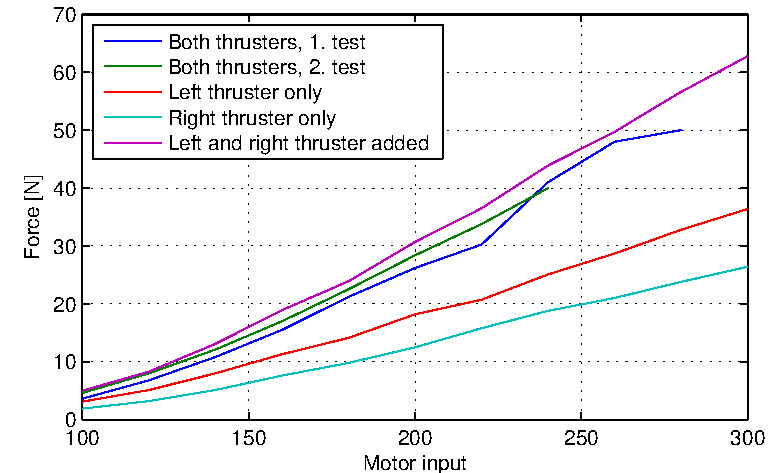
\includegraphics[width=0.6\textwidth]{plot/forwardthrust}
	\caption{Forward motion tests.}
	\label{fig:bollpullforward}
\end{figure}

\begin{figure}[htbp]
	\centering
	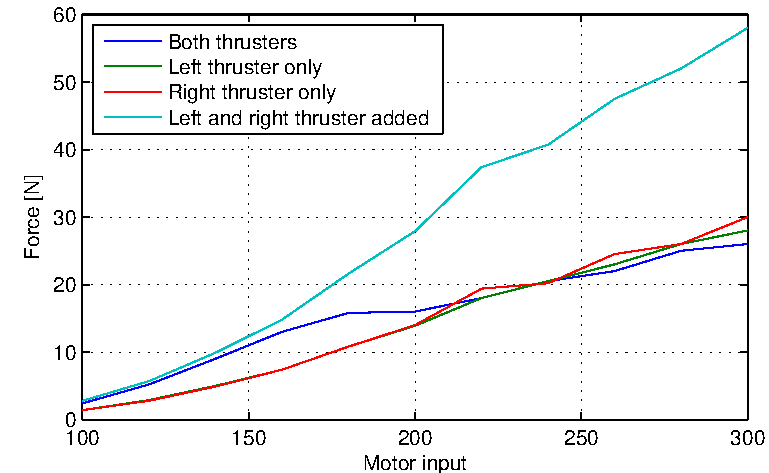
\includegraphics[width=0.6\textwidth]{plot/backthrust}
	\caption{Backward motion tests.}
	\label{fig:bollpullbackward}
\end{figure}

\begin{figure}[htbp]
	\centering
	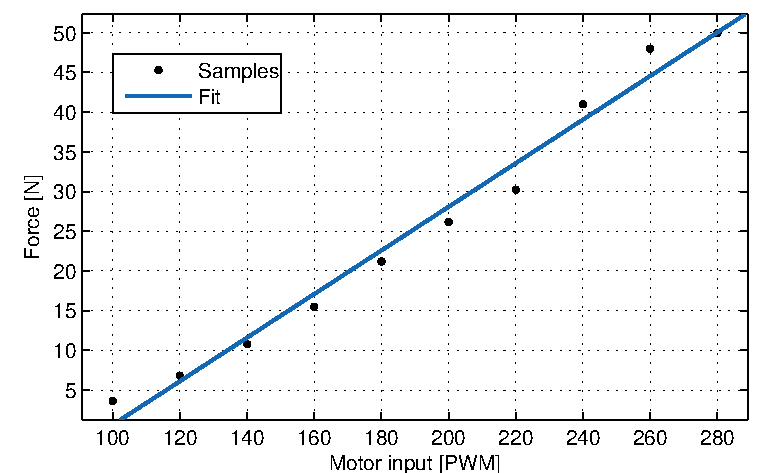
\includegraphics[width=0.6\textwidth]{plot/both_force_1_1order}
	\caption{Forward motion test with 1 order polynomial fitting.}
	\label{fig:1_1order}
\end{figure}

\begin{figure}[htbp]
	\centering
	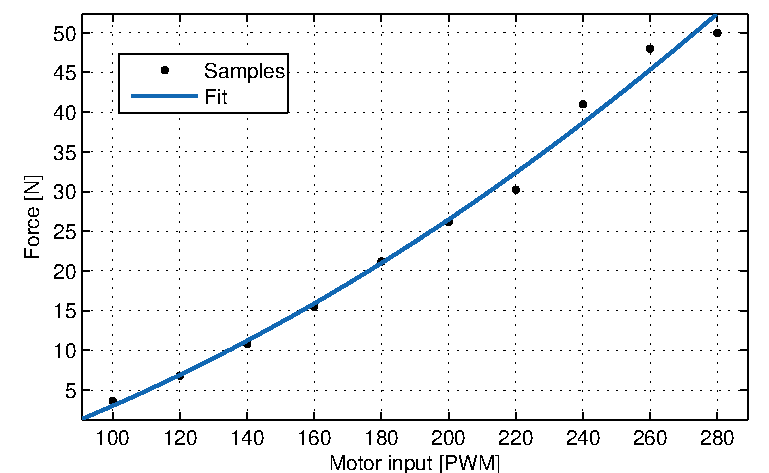
\includegraphics[width=0.6\textwidth]{plot/both_force_1_2order}
	\caption{Forward motion test with 2 order polynomial fitting.}
	\label{fig:1_2order}
\end{figure}

\begin{figure}[htbp]
	\centering
	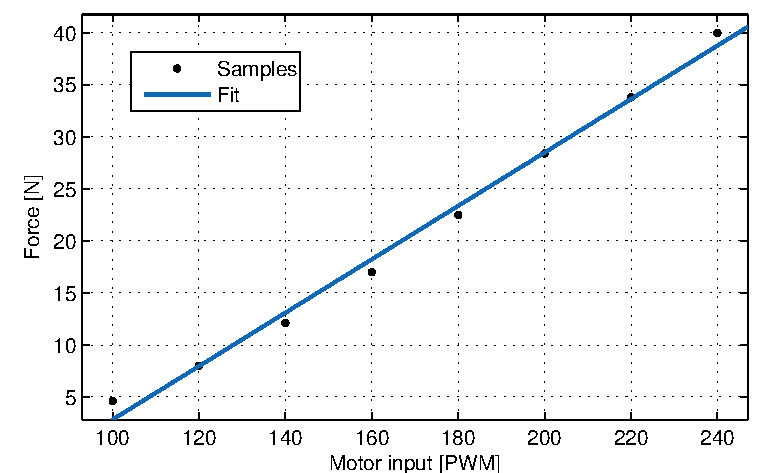
\includegraphics[width=0.6\textwidth]{plot/both_force_2_1order}
	\caption{Forward motion test with 1 order polynomial fitting.}
	\label{fig:2_1order}
\end{figure}

\begin{figure}[htbp]
	\centering
	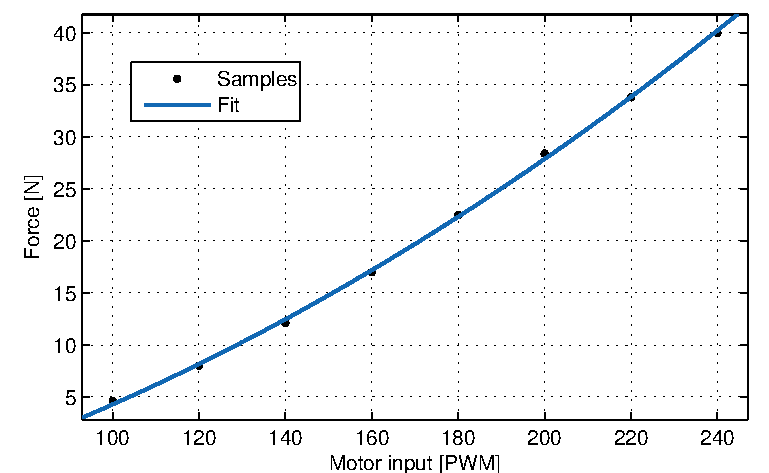
\includegraphics[width=0.6\textwidth]{plot/both_force_2_2order}
	\caption{Forward motion test with 2 order polynomial fitting.}
	\label{fig:2_2order}
\end{figure}

\begin{figure}[htbp]
	\centering
	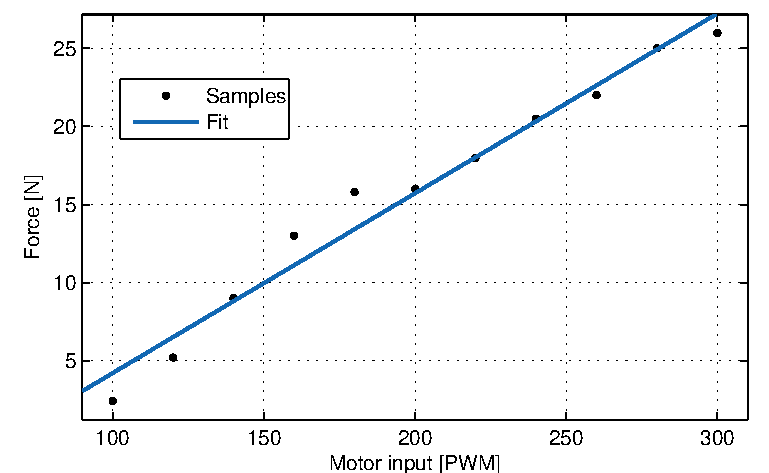
\includegraphics[width=0.6\textwidth]{plot/both_force_3_1order}
	\caption{Backward motion test with 1 order polynomial fitting.}
	\label{fig:3_1order}
\end{figure}

\begin{figure}[htbp]
	\centering
	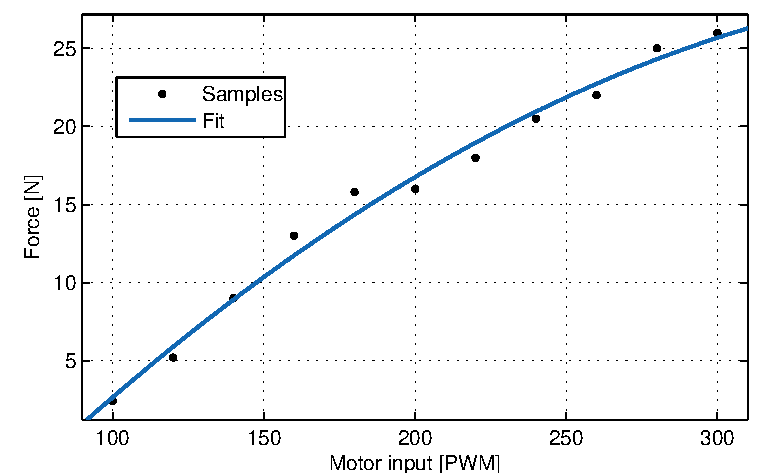
\includegraphics[width=0.6\textwidth]{plot/both_force_3_2order}
	\caption{Backward motion test with 2 order polynomial fitting.}
	\label{fig:3_2order}
\end{figure}

\begin{table}[htbp]
\centering
\begin{tabular}{cccc}
	\toprule
  Test & $R^2$ & RMSE & Function\\
  \midrule
  Both thrusters, forward \ref{fig:1_1order} & 0.9824 & 2.3626 & $f(x)=0.2746\cdot x-26.84$\\
  Both thrusters, forward \ref{fig:1_2order} & 0.9906 & 1.8414 & $f(x)=0.0004976\cdot x^2+0.08552\cdot x-10.52$\\
  Both thrusters, forward \ref{fig:2_1order} & 0.9929 & 1.1513 & $f(x)=0.2567\cdot x-22.83$\\
  Both thrusters, forward \ref{fig:2_2order} & 0.9994 & 0.3638 & $f(x)=0.0005208\cdot x^2+0.07958\cdot x-8.875$\\
  Both thrusters, backward \ref{fig:3_1order} & 0.9729 & 1.345 & $f(x)=0.1152\cdot x-7.318$\\
  Both thrusters, backward \ref{fig:3_1order} & 0.9883 & 0.9383 & $f(x)=-0.0002593\cdot x^2+0.2189\cdot x-16.65$\\
  \bottomrule
\end{tabular}
\caption{Coefficient of determination, Root Mean Square Error and the functions to the fittings.}
\label{tab:fitting}
\end{table}

\section{Discussion and Conclusion}
The fitting maps from motor \ac{PWM} input to force output in $N$. When looking at the two first regressions at the forward motion it can be chosen to either use the first order fitting or the second order fitting. The coefficient of determination and the RMSE does not deviate much from the samples in either cases. Thus it is concluded that the first order fitting can be as good as the second order fitting, and the first order is chosen as fitting.

When looking at the regression for the backward motion it can be seen, that the second order fitting estimates the $a$ coefficient of the fitting to be negative. This is due to the backward test. At a \ac{PWM} input above 160 is applied, the vessel starts to ventilate from the propellers. This makes the force, which the vessel's pulls with, be lesser than it actually would if it did not ventilate. Therefore is the first order also seen as the most reliable while going backwards.
